N?r det kommer til SMS beskeder, s? er der en gr?nse p? hvor mange tegn der kan v?re i en enkelt besked. For det latinske alfabet ligger begr?nsningen p? 160 tegn. Begr?nsningen ?ndrer sig fra tegns?t til tegns?t. For eksempel har det kinesiske alfabet en tegnbegr?nsning p? 70 tegn.\cite{Pro_1} Normalt vil en besked som fylder mere end sin tegnbegr?nsning blive delt op i to separate beskeder, hvis afsenderen af beskeden ikke selv g?r det, hvilket kommer til at betyde dobbelt SMS takst. Med denne begr?nsning i tankerne kommer sp?rgsm?let: Hvor betydeligt er dette problem, og er det overhovedet v?rd at kigge n?rmere p??
Erhvervs priserne for at sende en SMS inden for Norden og Eurozonen er betydeligt billigere end hvis man sendte til eller fra et Europa land ikke inde under EU, og n?r man sender til eller fra lande udenfor Europa s? bliver det kun dyrere og dyrere. Et internationalt firma som udnytter SMS til intern kommunikation eller andet kan ende med at bruge mange penge p? deres telefonregninger. Tilbage i 2009/2010 begyndte de forskellige telefonselskaber at h?ve prisen p? afsendelse af beskeder til udlandet. TDC's pris, for eksempel, gik fra at v?re p? 2,40 kr. til at koste 3,20 kr. per SMS.\cite{Pro_2} Nedenst?ende tabel viser Telenors SMS takst samt minutpris for erhverv.\cite{Pro_3}.

%\noindent
\begin{figure}[H]
\centering
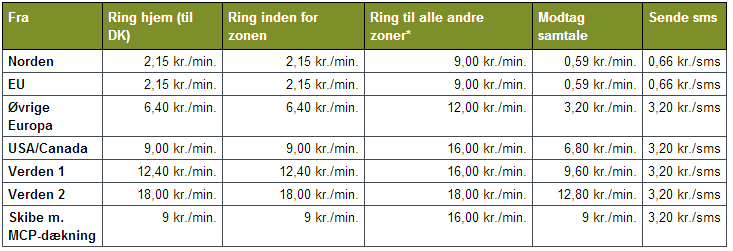
\includegraphics[width=\linewidth]{Billeder/Priser}
\caption {Telenor's SMS takst og minutpris for erhverv}
\centering
\end{figure}


Ligeledes er priserne for private hen over landegr?nserne heller ikke noget at prale af. I det private str?kker priserne sig fra 3's pris pr. SMS p? 2,50 kr\cite{Pro_4} til Telia's pris pr. SMS p? 4,00 kr.\cite{Pro_5} Uanset om man er privat eller erhvervsdrivende s? vil man gerne v?re sparsomme med antallet af beskeder man sender over landegr?nserne, og derudfra g?re god brug af sine 160 tegn s?dan at man undg?r dobbelt SMS takst ved at beskeden bliver delt i to.
Derfor vil en eller anden datalogisk l?sning, som g?r det lettere at sende beskede, uden at man skal bekymre som om hvorvidt ens besked har mere end de begr?nsede 160 tegn, v?re aktuelt. S?dan en l?sning kan b?de g?re det mere bekvemt for brugeren at bruge SMS'er, og i det lange l?b sparer brugeren penge.